\documentclass{article}
\usepackage[utf8]{inputenc}
\usepackage{amsmath}
\usepackage{graphicx}
\usepackage{hyperref}
\usepackage[hscale = 0.8, vscale = 0.9]{geometry}
\title{Modelling an epidemic by S.I.R model}
\date{}
\begin{document}
\pagenumbering{gobble}
\maketitle
\section*{What is the S.I.R model?}
The S.I.R model is a mathematical model that is used to study the spread of an epidemic, by theoretically computing the number of infected people with respect to time.



In this model, people are grouped into 3 categories :
\begin{itemize}
    \item People who are \emph{susceptible} to infection - those who are capable of getting infected (S)
    \item People who have got \emph{infected} (I)
    \item People who got infected and \emph{recovered} (R)
\end{itemize}


\section*{Assumptions of the S.I.R model}
\begin{itemize}
    \item A person can belong to only one category at any time. For instance, if a person if infected, they are no longer susceptible.
    \item  The epidemic can affect all people. Everyone is susceptible initially.
    \item Once a person is recovered, they gain immunity against the infection. They are no longer susceptible. They get infected only once.
    \item These three categories encompass everyone. The total population is also a constant. That is death due to the epidemic or otherwise is low
    \item Infection spreads only by contact between susceptible and infected persons.
\end{itemize}    
\section*{Mathematics involved and explanation of model} 
Let $S(t)$ be the number of susceptible people as a function of time, $I(t)$ be the number of infected people and $R(t)$ be the recovered people. From the assumptions, $S(t) + I(t) + R(t) = N$, where $N$ is the total population - a constant.

A susceptible person becomes infected when he comes in contact with an infected person. The number of interactions between them will be proportional to both the number of infected as well as number of susceptible people. Higher the population of these 2 categories, more is the chance of contact, higher is the chance of infection.

Hence, people get infected at a rate $a\cdot S(t)\cdot I(t)$, where a is a positive constant of proportionality. Numerically, $$\frac{dS}{dt} = -a\cdot S\cdot I$$ As people get infected, they leave the susceptible category and enter the infected category. Hence the minus sign.

People enter the infected category at a rate of $a\cdot S\cdot I$. But that is not the only factor affecting it. People get recovered too. We assume that more is the number of infected people, more would be the recovery rate, i.e recovery rate $\propto$ I(t).

Thus, $$\frac{dI}{dt}=\left(a\cdot S\cdot I - b\cdot I\right)\textrm {  and } \frac{dR}{dt} = b\cdot I$$ where b is a positive constant of proportionality.
\pagebreak

We have the equations :
\begin{align}
    \frac{dS}{dt} = -a\cdot S\cdot I
\end{align}
\begin{align}
    \frac{dI}{dt} = a\cdot S \cdot I - b\cdot I
\end{align}
\begin{align}
    \frac{dR}{dt} = b\cdot I
\end{align}

This set of three equations are an example of simultaneous system of differential equations. As there is a product term $S\cdot I$ involved in these equations, its solution is not trivial, but we can still do some analysis just with these derivative equations.

\section*{Some simple analysis}
\subsection*{Near time = 0:}
Let $S_0$ be the initial susceptible people, $I_0$ be the initial number of infected people. At the start of an epidemic, number of recovered people is 0.

At the start of an epidemic, the number of infected people is small (we detect the infection when number of infected people is low). Hence, $I_0$ is very low and correspondingly, $S_0$ is quite high.
\subsubsection*{An introduction to R_0 :}
$\frac{dI}{dt} \textrm{ at } t = 0 \textrm{ is } (a\cdot S_0 \cdot I_0 -b \cdot I_0) $. 
An aspect of interest would be to see if we will have an epidemic or not. This is determined by the sign of $\frac{dI}{dt} $ at t = 0. If it is less than 0, it means people recover faster than they get infected, thus the infected population becomes 0 even before it can increase. If it is greater than 0, there is a net spread of disease, hence there will be an epidemic.

So we ask "is $(a\cdot S_0 - b)\cdot I_0 < 0$?". This amounts to asking if $$\frac{a \cdott S_0}{b} < 1.$$ This expression $\frac{a\cdot S_0}{b}$ is called $R_0$. 
\begin{itemize}
    \item If $R_0 < 1$, then the number of infected people reach 0 even before there is considerable spread, thus preventing an epidemic.
    \item Even if $R_0 > 1$, a low value of $R_0$ is preferred over a higher value. A high value means that the spread of infection is fast, which isn't desirable.
\end{itemize}
Factors affecting $R_0$ : 
\begin{itemize}
    \item $R_0$ is directly proportional to a, the proportionality constant pertaining to infection rate. When we do practices like preventing contact by social distancing, isolating the infected, washing hands and face regularly, we can reduce this a, hence reducing $R_0$. This is the idea of flattening the curve in a nutshell!
    \item We can also decrease $S_0$ by bringing vaccines into the picture. Vaccines bring about immunity from the disease, thus making them insusceptible.
    \item We cannot really affect b, unless we find a cure and improve healthcare to increase b.
\end{itemize}
\subsubsection*{I(t) near t = 0 :}
S is quite high near this initial part of epidemic. We can roughly say that S is always $S_0$ near t = 0.
Hence, we have the differential equation $\frac{dI}{dt} \approx I\cdot(a\cdot S_0 - b)$. 

$I(t)$ has the solution $ I(t) \approx e^{\left(a\cdot S_0 - b\right)t} $. \emph{I(t) roughly follows an exponential solution near the start of an epidemic.}

\subsection*{Rough graphs of S(t), I(t) and R(t) :}
\begin{itemize}
    \item S(t) : Initially, everyone is susceptible and hence $S_0$ is close to N. As time progresses, S keeps decreasing as more and more get infected and after a point, everyone would have been infected, making S to be 0.
    \item I(t) : Initially, number of infected people is low, but it increases due to the $a\cdot S \cdot I$ term. Over time, I keeps increasing. However, after a point, the $-b \cdot I$ term increases and it begins to dominate. I(t) reaches a peak and then decreases and eventually becomes 0 as people recover over time.
    \item R(t) : The recovered people starts at 0 and keeps increasing. It keeps increasing at a rate proportional to infected people. After a point, everyone would have been infected and reached the recovered stage.
    
    A rough graph illustrating these points is shown in \ref{fig:sir_graph}
\end{itemize}    
\begin{figure}
    \centering
    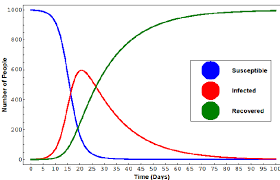
\includegraphics[scale = 1.00]{sir}
    \caption{A model S.I.R graph. (Image taken from the net.)}
    \label{fig:sir_graph}
\end{figure}
\section*{Improvements and variants of the S.I.R model : }
The S.I.R model is quite simple and not always representative of an actual epidemic. Several improvements can be added. Some are :
\begin{itemize}
    \item Vital dynamics : We have to account for births and deaths as well. We can incorporate a birth and death rates. The total population too can fluctuate.
    \item S.E.I.R model : Sometimes, we don't get infected as soon as we contact an infected person. There is usually some latency period. We can introduce a new category called "exposed" people, who are in this latency period. They will spread the infection at a rate lower than people who are actually infected.
    \item S.I.S model : Sometimes, we don't actually recover even after getting infected. We can get infected again. We can use the S.I.S model, which is the susceptible, infected, cured-yet-susceptible model. Common cold is one such infection. It is also possible that some get immunity and some don't, depending on how good their immune system is. 
\end{itemize}    
A good model for an epidemic would be one which incorporates all these ideas. However, it is worth mentioning that the equations and solutions will get more complicated.
\section*{References}
\begin{enumerate}
    \item \url{https://youtu.be/Qrp40ck3WpI}
    \item \url{https://youtu.be/f1a8JYAixXU}
    \item \url{https://en.wikipedia.org/wiki/Compartmental_models_in_epidemiology#The_SIRV_model}
\end{enumerate}




\end{document}


